\chapter{Dashboard}

\section{Dashboard Overview}

The KanardiaCloud dashboard serves as your central control center, providing an at-a-glance view of all important information and quick access to frequently used features.

\begin{figure}[H]
\centering
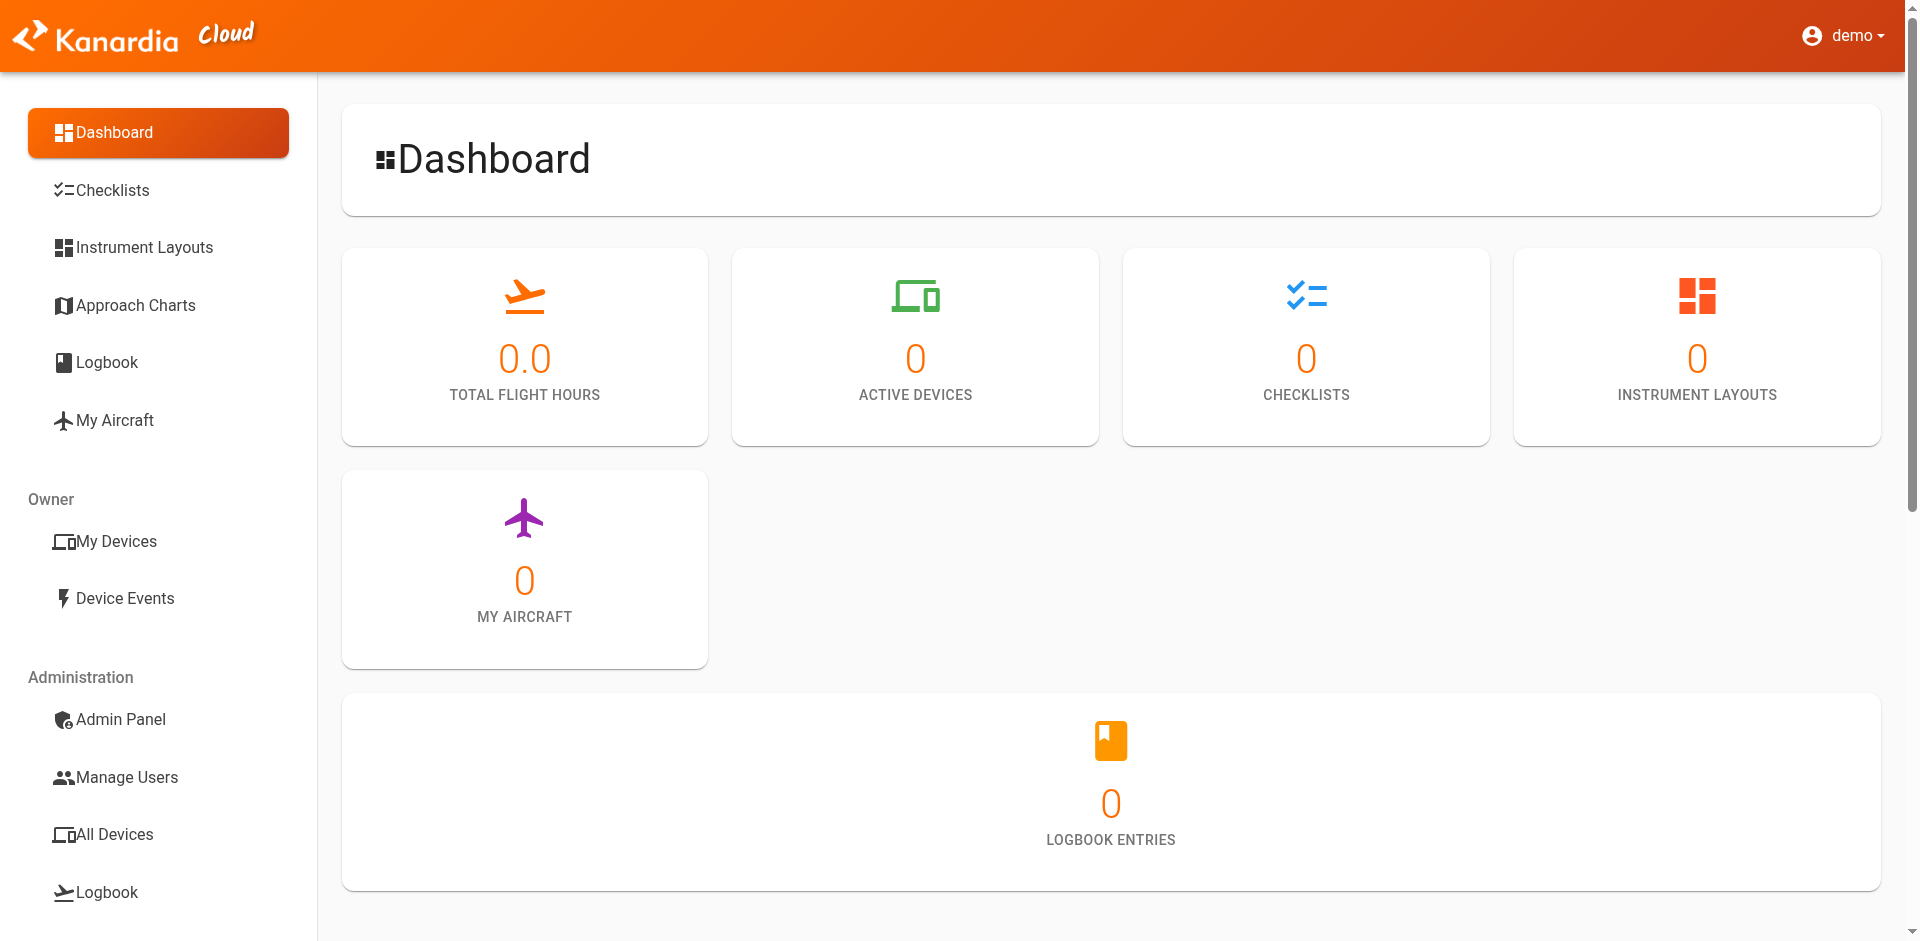
\includegraphics[width=\textwidth]{images/main_dashboard.png}
\caption{KanardiaCloud Main Dashboard}
\label{fig:main_dashboard}
\end{figure}

\section{Dashboard Components}

\subsection{Header Navigation}

The top header contains:

\begin{itemize}
    \item \textbf{Logo}: Click to return to dashboard
    \item \textbf{Main Navigation}: Access all major sections
    \item \textbf{User Menu}: Profile, settings, and logout options
    \item \textbf{Notifications}: System alerts and updates
\end{itemize}

\subsection{Quick Statistics}

Key metrics displayed prominently:

\begin{table}[H]
\centering
\begin{tabular}{@{}lp{8cm}@{}}
\toprule
\textbf{Metric} & \textbf{Description} \\
\midrule
Connected Devices & Number of active Kanardia devices \\
Total Flight Hours & Cumulative flight time from logbook \\
Active Checklists & Number of available checklists \\
Recent Flights & Last 7 days flight activity \\
System Status & Overall system health indicator \\
\bottomrule
\end{tabular}
\caption{Dashboard Quick Statistics}
\label{tab:dashboard_stats}
\end{table}

\subsection{Recent Activity}

The activity feed shows:
\begin{itemize}
    \item Recent logbook entries
    \item Checklist modifications
    \item Device synchronization events
    \item System notifications
    \item User actions and changes
\end{itemize}

\subsection{Quick Actions Panel}

One-click access to common tasks:
\begin{itemize}
    \item Add new flight entry
    \item Create checklist
    \item Connect new device
    \item Upload approach chart
    \item Generate reports
\end{itemize}

\section{Customization}

\subsection{Widget Configuration}

Customize your dashboard by:
\begin{enumerate}
    \item Clicking the settings icon in the top-right
    \item Selecting which widgets to display
    \item Arranging widget order
    \item Setting refresh intervals
    \item Configuring data ranges
\end{enumerate}

\subsection{Personal Preferences}

Set your preferences for:
\begin{itemize}
    \item Default date/time formats
    \item Measurement units (metric/imperial)
    \item Language settings
    \item Theme preferences
    \item Notification settings
\end{itemize}
